
\paragraph{The correctness of distributed algorithms} is the focus of this thesis. Distributed algorithms
are algorithms that are designed to run on multiple processors, without centralized control. They play a crucial role in modern computing.
For example, they control machines that we use on a daily basis such as smartphones, but also critical systems such as medical devices, trains, airplanes, and spaceships. Errors in distributed algorithms can have severe consequences, such as the loss of critical data or even the loss of human life. Ensuring their correctness is vital but challenging due to the inherent complexity of these systems~\cite{heiser2010theroad, lamport2019thebyzantine}. For example, the Needham Schroeder public key protocol~\cite{needham1978using}, which is intended to provide mutual authentication between two parties communicating on a network, has been shown to have vulnerabilities that can be exploited by attackers~\cite{lowe1996breaking}, 17 years after the publication of the original paper~\cite{cortier2014formal}.

% While interactive theorem proving~\cite{harrison2014history}\textemdash a method where humans guide specialized softwares, called proof assistants, to construct formal mathematical proofs step-by-step\textemdash offers a promising approach to formally verifying properties of distributed systems~\cite{plump2024formalisingDPO,potop2019formal,courtieu2016certified},  
% it requires proficiency in proof assistants and can be
% time-consuming.

% \paragraph{Interactive theorem proving (ITP)}~\cite{harrison2014history,itp2016}
% offers a rigorous approach to address these challenges~\cite{courtieu2022swarms}. 
% In ITP, humans collaborate with proof assistants~\cite{nipkow2002isabelle, bertot2004coq, moura2021lean4}—specialized software tools—to construct formal mathematical proofs step-by-step. 
% Specifically, objects such as distributed algorithms can be modeled as mathematical objects, and properties of these objects can be expressed as mathematical statements.
% We guide proof assistants to construct formal proofs of these statements by providing reasoning steps to the proof assistants, and proof assistants check the correctness of these steps.

\paragraph{Interactive theorem proving (ITP)}
% ~\cite{harrison2014history,itp2016} 
provides a rigorous framework for formal verification through human-guided collaboration with proof assistants~\cite{nipkow2002isabelle,bertot2004coq,moura2021lean4}. In this paradigm, distributed algorithms are formally modeled as mathematical structures, with their properties expressed as logical statements. The verification process involves guiding proof assistants through a sequence of inference steps, with the system rigorously checking each transition for correctness.

This approach has proven effective for verifying critical properties of distributed systems~\cite{plump2024formalisingDPO,potop2019formal,courtieu2016certified}.
However, ITP presents significant challenges: it demands expertise in proof assistants because it requires a deep understanding of both the system being verified and the proof assistant being used, and the proof construction process remains inherently labor-intensive because the proof assistant must be guided through each step of the reasoning process and every possible case must be considered in detail.
 While modern proof assistants incorporate increasingly sophisticated automation for specific proof patterns, fundamental limitations arise from the undecidability of the underlying logics required for expressiveness.
 Consequently, complete automation of proof construction for non-trivial distributed systems remains theoretically impossible—though strategic advances in proof engineering and domain-specific tactics continue to reduce the human effort required for verification.

\paragraph{Automated methods} that check specific properties of distributed algorithms and can generate certificates that can be checked by proof assistants provide a practical alternative~\cite{contejean2011automated,giesl2014proving}. While they can only be applied to specific properties for some classes of distributed algorithms, they can be used by users who are not experts in formal methods, and they can also speed up the verification process for experts. To develop such automated methods, distributed algorithms need to be modeled in a formal way enabling rigorous analysis and automated verification of their properties. In this thesis, we focus on modeling distributed algorithms using graph transformation.

 \paragraph{Rule-based graph transformation} provides an intuitive yet formal way to model distributed systems: computation units are represented by nodes; communication canals are represented by edges; states of the system are modeled by graphs whose edges have labels representing information encoded in computation units and states of communication canals; state changes of the system are modeled by replacing subgraphs in the graph by other subgraphs according to transformation rules. For example, consider the graph in~\autoref{fig:graph_modeling_state_network} which models a distributed network with six computation units. Each node represents a computation unit, with labels indicating their states: one unit is active ("A") while the remaining five are neutral ("N"). Edges represent communication canals, all initially in state "0". Consider a distributed spanning tree construction algorithm: when an active unit ("A") detects a neutral neighbor ("N") via a canal in state "0", it activates the neighbor and updates the canal to state "1". Its behavior can be captured by a graph transformation rule, which replaces the subgraph \tikz[baseline=0ex]{ 
            \node (x) at (0,0) {$\bullet$};  
            \node (y) at (1,0) {$\bullet$};
            \draw[-] (x) -- node[midway,above] {0} (y) ;
            \node () at (0,0.3) {$A$};  
            \node () at (1,0.3) {$N$};
     } by \tikz[baseline=0ex]{ 
                \node (x) at (0,0) {$\bullet$};  
                \node (y) at (1,0) {$\bullet$};
                \draw[-] (x) -- node[midway,above] {1} (y) ;
                \node () at (0,0.3) {$A$};  
                \node () at (1,0.3) {$A$};
     }. 
A sample execution sequence starting from the configuration in~\autoref{fig:graph_modeling_state_network} is shown in~\autoref{fig:intro_sequence_of_transformation}. Upon termination, a spanning tree can be constructed using edges labeled by "1".
 \begin{figure}
        \centering
        \resizebox{0.3\textwidth}{!}{
                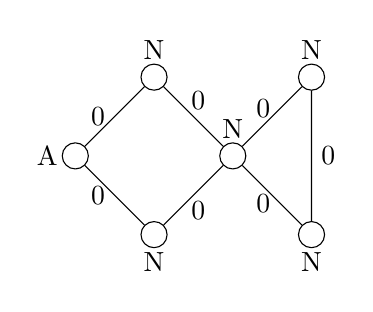
\begin{tikzpicture}
                    \node[draw, circle] (n1) at (0,0) {};
                    \node[draw, circle] (n2) at (1,1) {};
                    \node[draw, circle] (n4) at (1,-1) {};
                    \node[draw, circle] (n3) at (2,0) {};
                    \node[draw, circle] (n5) at (3,-1){};
                    \node[draw, circle] (n6) at (3,1){};
                    \draw[-] (n1)--(n2)--(n3)--(n4);
                    \draw[-] (n4)--(n1);
                    \draw[-] (n3)--(n6)--(n5)--(n3);
                    \draw[transparent, rounded corners,rotate around={45:(0,-0.5)}, dotted] (0,-0.5) rectangle (2.2,0.3) ;
                    \draw[transparent, rounded corners,rotate around={-45:(0,0.5)}, dotted] (0,0.5) rectangle (2.2,-0.3) ;   
                    \draw(-0.1,0) node[left] {A};
                    \draw(1,1.1) node[above] {N};
                    \draw(1,-1.1) node[below] {N};
                    \draw(2,0.1) node[above] {N};
                    \draw(3,1.1) node[above] {N};
                    \draw(3,-1.1) node[below] {N};
                    % edge labels
                    \draw(1.35,0.7) node[right] {0};
                    \draw(1.35,-0.7) node[right] {0};
                    \draw(0.5,0.5) node[left] {0};
                    \draw(0.5,-0.5) node[left] {0};
                    \draw(2.6,0.6) node[left] {0};
                    \draw(2.6,-0.6) node[left] {0};
                    \draw(3,0) node[right] {0};
                \end{tikzpicture}
    }
    \caption{A graph modeling a network configuration}
    
    \label{fig:graph_modeling_state_network}
    \end{figure}
    \begin{figure}
        \centering
        \resizebox{0.3\textwidth}{!}{
                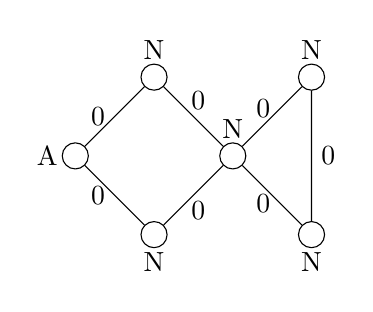
\begin{tikzpicture}
                    \node[draw, circle] (n1) at (0,0) {};
                    \node[draw, circle] (n2) at (1,1) {};
                    \node[draw, circle] (n4) at (1,-1) {};
                    \node[draw, circle] (n3) at (2,0) {};
                    \node[draw, circle] (n5) at (3,-1){};
                    \node[draw, circle] (n6) at (3,1){};
                    \draw[-] (n1)--(n2)--(n3)--(n4);
                    \draw[-] (n4)--(n1);
                    \draw[-] (n3)--(n6)--(n5)--(n3);
                    \draw[transparent, rounded corners,rotate around={45:(0,-0.5)}, dotted] (0,-0.5) rectangle (2.2,0.3) ;
                    \draw[transparent, rounded corners,rotate around={-45:(0,0.5)}, dotted] (0,0.5) rectangle (2.2,-0.3) ;   
    
                    \draw(-0.1,0) node[left] {A};
                    \draw(1,1.1) node[above] {N};
                    \draw(1,-1.1) node[below] {N};
                    \draw(2,0.1) node[above] {N};
                    \draw(3,1.1) node[above] {N};
                    \draw(3,-1.1) node[below] {N};
    
                    % edge labels
                    \draw(1.35,0.7) node[right] {0};
                    \draw(1.35,-0.7) node[right] {0};
                    \draw(0.5,0.5) node[left] {0};
                    \draw(0.5,-0.5) node[left] {0};
                    \draw(2.6,0.6) node[left] {0};
                    \draw(2.6,-0.6) node[left] {0};
                    \draw(3,0) node[right] {0};
                \end{tikzpicture}
    }
  \resizebox{0.3\textwidth}{!}{
                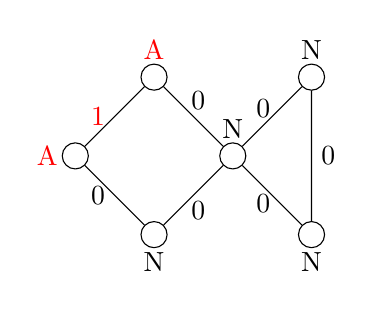
\begin{tikzpicture}
                    \node[draw, circle] (n1) at (0,0) {};
                    \node[draw, circle] (n2) at (1,1) {};
                    \node[draw, circle] (n4) at (1,-1) {};
                    \node[draw, circle] (n3) at (2,0) {};
                    
                    \node[draw, circle] (n5) at (3,-1){};
                    \node[draw, circle] (n6) at (3,1){};
        
                    \draw[-] (n1)--(n2)--(n3)--(n4);
                    \draw[-] (n4)--(n1);
                    \draw[-] (n3)--(n6)--(n5)--(n3);
        
                    \draw[transparent, rounded corners,rotate around={45:(0,-0.5)}, dotted] (0,-0.5) rectangle (2.2,0.3) ;
                    \draw[transparent, rounded corners,rotate around={-45:(0,0.5)}, dotted] (0,0.5) rectangle (2.2,-0.3) ;
    
                    \draw(-0.1,0) node[left] {\textcolor{red}{A}};
                    \draw(1,1.1) node[above] {\textcolor{red}{A}};
                    \draw(1,-1.1) node[below] {N};
                    \draw(2,0.1) node[above] {N};
                    \draw(3,1.1) node[above] {N};
                    \draw(3,-1.1) node[below] {N};
    
                    % edge labels
                    \draw(1.35,0.7) node[right] {0};
                    \draw(1.35,-0.7) node[right] {0};
                    \draw(0.5,0.5) node[left] {\textcolor{red}{1}};
                    \draw(0.5,-0.5) node[left] {0};
                    \draw(2.6,0.6) node[left] {0};
                    \draw(2.6,-0.6) node[left] {0};
                    \draw(3,0) node[right] {0};
                \end{tikzpicture}
}
\resizebox{0.3\textwidth}{!}{
                    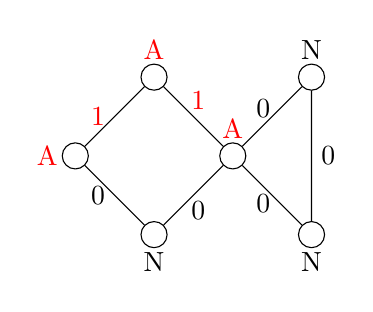
\begin{tikzpicture}
                        \node[draw, circle] (n1) at (0,0) {};
                        \node[draw, circle] (n2) at (1,1) {};
                        \node[draw, circle] (n4) at (1,-1) {};
                        \node[draw, circle] (n3) at (2,0) {};
                        
                        \node[draw, circle] (n5) at (3,-1){};
                        \node[draw, circle] (n6) at (3,1){};
            
                        \draw[-] (n1)--(n2)--(n3)--(n4);
                        \draw[-] (n4)--(n1);
                        \draw[-] (n3)--(n6)--(n5)--(n3);
            
                        \draw[transparent, rounded corners,rotate around={45:(0,-0.5)}, dotted] (0,-0.5) rectangle (2.2,0.3) ;
                        \draw[transparent, rounded corners,rotate around={-45:(0,0.5)}, dotted] (0,0.5) rectangle (2.2,-0.3) ;
    
                        \draw(-0.1,0) node[left] {\textcolor{red}{A}};
                        \draw(1,1.1) node[above] {\textcolor{red}{A}};
                        \draw(1,-1.1) node[below] {N};
                        \draw(2,0.1) node[above] {\textcolor{red}{A}};
                        \draw(3,1.1) node[above] {N};
                        \draw(3,-1.1) node[below] {N};
    
                        % edge labels
                        \draw(1.35,0.7) node[right] {\textcolor{red}{1}};
                        \draw(1.35,-0.7) node[right] {0};
                        \draw(0.5,0.5) node[left] {\textcolor{red}{1}};
                        \draw(0.5,-0.5) node[left] {0};
                        \draw(2.6,0.6) node[left] {0};
                        \draw(2.6,-0.6) node[left] {0};
                        \draw(3,0) node[right] {0};
                    \end{tikzpicture}
}


\resizebox{0.3\textwidth}{!}{
                    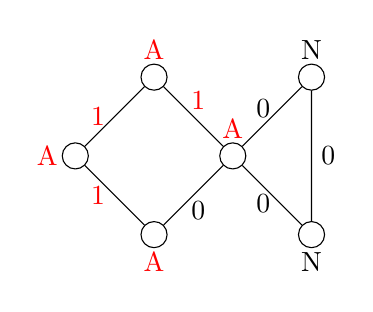
\begin{tikzpicture}
                        \node[draw, circle] (n1) at (0,0) {};
                        \node[draw, circle] (n2) at (1,1) {};
                        \node[draw, circle] (n4) at (1,-1) {};
                        \node[draw, circle] (n3) at (2,0) {};
                        
                        \node[draw, circle] (n5) at (3,-1){};
                        \node[draw, circle] (n6) at (3,1){};
            
                        \draw[-] (n1)--(n2)--(n3)--(n4);
                        \draw[-] (n4)--(n1);
                        \draw[-] (n3)--(n6)--(n5)--(n3);
            
                        \draw[transparent, rounded corners,rotate around={45:(0,-0.5)}, dotted] (0,-0.5) rectangle (2.2,0.3) ;
                        \draw[transparent, rounded corners,rotate around={-45:(0,0.5)}, dotted] (0,0.5) rectangle (2.2,-0.3) ;
    
                        \draw(-0.1,0) node[left] {\textcolor{red}{A}};
                        \draw(1,1.1) node[above] {\textcolor{red}{A}};
                        \draw(1,-1.1) node[below] {\textcolor{red}{A}};
                        \draw(2,0.1) node[above] {\textcolor{red}{A}};
                        \draw(3,1.1) node[above] {N};
                        \draw(3,-1.1) node[below] {N};
    
                        % edge labels
                        \draw(1.35,0.7) node[right] {\textcolor{red}{1}};
                        \draw(1.35,-0.7) node[right] {0};
                        \draw(0.5,0.5) node[left] {\textcolor{red}{1}};
                        \draw(0.5,-0.5) node[left] {\textcolor{red}{1}};
                        \draw(2.6,0.6) node[left] {0};
                        \draw(2.6,-0.6) node[left] {0};
                        \draw(3,0) node[right] {0};
                    \end{tikzpicture}
}
\resizebox{0.3\textwidth}{!}{
                    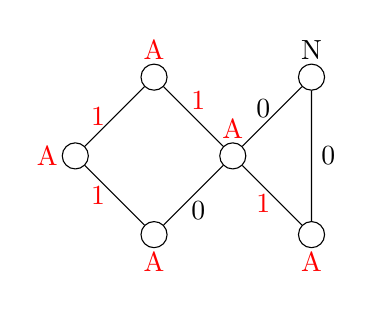
\begin{tikzpicture}
                        \node[draw, circle] (n1) at (0,0) {};
                        \node[draw, circle] (n2) at (1,1) {};
                        \node[draw, circle] (n4) at (1,-1) {};
                        \node[draw, circle] (n3) at (2,0) {};
                        
                        \node[draw, circle] (n5) at (3,-1){};
                        \node[draw, circle] (n6) at (3,1){};
            
                        \draw[-] (n1)--(n2)--(n3)--(n4);
                        \draw[-] (n4)--(n1);
                        \draw[-] (n3)--(n6)--(n5)--(n3);
            
                        \draw[transparent, rounded corners,rotate around={45:(0,-0.5)}, dotted] (0,-0.5) rectangle (2.2,0.3) ;
                        \draw[transparent, rounded corners,rotate around={-45:(0,0.5)}, dotted] (0,0.5) rectangle (2.2,-0.3) ;
              
                        \draw(-0.1,0) node[left] {\textcolor{red}{A}};
                        \draw(1,1.1) node[above] {\textcolor{red}{A}};
                        \draw(1,-1.1) node[below] {\textcolor{red}{A}};
                        \draw(2,0.1) node[above] {\textcolor{red}{A}};
                        \draw(3,1.1) node[above] {N};
                        \draw(3,-1.1) node[below] {\textcolor{red}{A}};
    
                        % edge labels
                        \draw(1.35,0.7) node[right] {\textcolor{red}{1}};
                        \draw(1.35,-0.7) node[right] {0};
                        \draw(0.5,0.5) node[left] {\textcolor{red}{1}};
                        \draw(0.5,-0.5) node[left] {\textcolor{red}{1}};
                        \draw(2.6,0.6) node[left] {0};
                        \draw(2.6,-0.6) node[left] {\textcolor{red}{1}};
                        \draw(3,0) node[right] {0};
                    \end{tikzpicture}
}
\resizebox{0.3\textwidth}{!}{
                    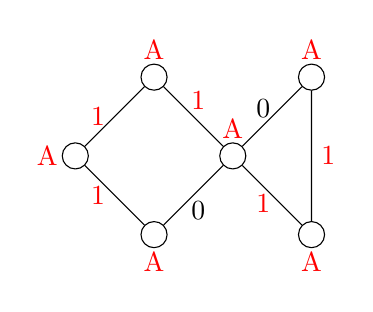
\begin{tikzpicture}
                        \node[draw, circle] (n1) at (0,0) {};
                        \node[draw, circle] (n2) at (1,1) {};
                        \node[draw, circle] (n4) at (1,-1) {};
                        \node[draw, circle] (n3) at (2,0) {};
                        
                        \node[draw, circle] (n5) at (3,-1){};
                        \node[draw, circle] (n6) at (3,1){};
            
                        \draw[-] (n1)--(n2)--(n3)--(n4);
                        \draw[-] (n4)--(n1);
                        \draw[-] (n3)--(n6)--(n5)--(n3);
            
                        \draw[transparent, rounded corners,rotate around={45:(0,-0.5)}, dotted] (0,-0.5) rectangle (2.2,0.3) ;
                        \draw[transparent, rounded corners,rotate around={-45:(0,0.5)}, dotted] (0,0.5) rectangle (2.2,-0.3) ;
                        \draw(-0.1,0) node[left] {\textcolor{red}{A}};
                        \draw(1,1.1) node[above] {\textcolor{red}{A}};
                        \draw(1,-1.1) node[below] {\textcolor{red}{A}};
                        \draw(2,0.1) node[above] {\textcolor{red}{A}};
                        \draw(3,1.1) node[above] {\textcolor{red}{A}};
                        \draw(3,-1.1) node[below] {\textcolor{red}{A}};
    
                        % edge labels
                        \draw(1.35,0.7) node[right] {\textcolor{red}{1}};
                        \draw(1.35,-0.7) node[right] {0};
                        \draw(0.5,0.5) node[left] {\textcolor{red}{1}};
                        \draw(0.5,-0.5) node[left] {\textcolor{red}{1}};
                        \draw(2.6,0.6) node[left] {0};
                        \draw(2.6,-0.6) node[left] {\textcolor{red}{1}};
                        \draw(3,0) node[right] {\textcolor{red}{1}};
                    \end{tikzpicture}
}
        \caption{A possible sequence of graph transformation}
        \label{fig:intro_sequence_of_transformation}
    \end{figure}

 Graph transformation has many applications, such as topology-based geometric modeling~\cite{poudret2007topology, belhaouari2014jerboa, bellet2017geometric, pascale2022Geometric_modeling}, DNA computing~\cite{harju2004tutorial_dna_computation}, and software engineers~\cite{heckel2020software_engineers}.
 
 A predominant school of thought in this area is called algebraic graph rewriting~\cite{ehrig1997handbook1,ehrig1999handbook2,ehrig1999handbook3} which uses concepts from category theory~\cite{pierce1991basic,barr1990category,maclane2013categories} to define the transformation of graphs. The language of category theory abstract away from the details of the different notions of graphs, provided that the notion of graph satisfies some properties~\cite{lack2004adhesive,overbeek2023graph}. 
 In fact, different notions of graphs have been proposed in the literature for different applications, such as edge-labeled multigraphs~\cite{konig2018atutorial,corradini1997algebraic}, hypergraphs~\cite{plump1993hypergraph}, attributed graphs~\cite{ehrig2006fundamentals}, etc. Another advantage is that transformation is defined up to isomorphism, which leads to a more elegant definition of graph transformation.

  To transform a host graph $G$ using a rule which replaces an occurrence of a graph $L$ in $G$ by the occurrence of another graph $R$, one firstly needs to decompose the host graph $G$ into a context $C$ and an occurrence of $L$, then removes some nodes and edges of the occurrence of $L$ and finally adds some fresh nodes and edges to form the result graph. For example, if we consider a graph transformation rule which identifies an occurrence of the following graph, then removes the middle node and edges of the occurrence and adds no fresh nodes and edges:
\begin{center}
    \begin{tikzpicture}
           \graphbox{\( \)}{0mm}{-3mm}{34mm}{12mm}{2mm}{2mm}{
                \coordinate (o) at (0mm,-8mm); 
                \node[draw,circle] (l1) at ($(o)+(-10mm,0mm)$) {1};
                \node[draw,circle] (l2) at ($(l1)+(2,0)$) {2};
                \node[draw,circle] (l3) at ($(l1) + (1,0)$) {3};
                \draw[->] (l1) -- (l3) node[midway,above] {a};
                \draw[->] (l3) -- (l2) node[midway,above] {a};
            } 
    \end{tikzpicture}
\end{center}
The graph $G$, illustrated below, can be transformed into the graph $H$, illustrated below, by applying the rule.
\begin{center}
  \begin{tikzpicture}
     \graphbox{\( G \)}{0mm}{-22mm}{34mm}{22mm}{2mm}{-3mm}{
              \coordinate (o) at (0mm,-3mm); 
              \node[draw,circle] (l1) at ($(o)+(-10mm,0mm)$) {1};
              \node[draw,circle] (l2) at ($(l1)+(2,0)$) {2};
              \node[draw,circle] (l3) at ($(l1) + (1,0)$) {3};
              \node[draw,circle] (l4) at ($(l2) + (0,-1)$) {6};
              \draw[] (l1) -- (l3) node[midway,above] {a};
              \draw[] (l3) -- (l2) node[midway,above] {a};
              \draw[ ] (l2) -- (l4) node[midway,right] {b};
              \node[draw,circle] (l6) at ($(l1) + (0,-1)$) {7};
              \draw[] (l1) -- (l6) node[midway,left] {b};
          }    
          \graphbox{\( H \)}{40mm}{-22mm}{34mm}{22mm}{2mm}{-3mm}{
              \coordinate (o) at (0mm,-3mm); 
              \node[draw,circle] (l1) at ($(o)+(-10mm,0mm)$) {1};
              \node[draw,circle] (l2) at ($(l1)+(2,0)$) {2};
              \node[draw,circle] (l4) at ($(l2) + (0,-1)$) {6};
              \draw[ ] (l2) -- (l4) node[midway,right] {b};
              \node[ draw,circle] (l6) at ($(l1) + (0,-1)$) {7};
              \draw[ ] (l1) -- (l6) node[midway,left] {b};
          }    
  \end{tikzpicture}
\end{center}
The problem arises when it comes to whether the rule mentioned above can be applied to the following graph $G'$ because of the edge in red:
\begin{center}
  \begin{tikzpicture}
    \graphbox{\( G' \)}{0mm}{-22mm}{34mm}{22mm}{2mm}{-3mm}{
                \coordinate (o) at (0mm,-3mm); 
                \node[draw,circle] (l1) at ($(o)+(-10mm,0mm)$) {1};
                \node[draw,circle] (l2) at ($(l1)+(2,0)$) {2};
                \node[draw,circle] (l3) at ($(l1) + (1,0)$) {3};
                \node[draw,circle] (l4) at ($(l2) + (0,-1)$) {6};
                \draw[->,red] (l3) -- (l4) node[midway,above] {a};
                \draw[->] (l1) -- (l3) node[midway,above] {a};
                \draw[->] (l3) -- (l2) node[midway,above] {a};
                \draw[->] (l2) -- (l4) node[midway,right] {b};
                \node[draw,circle] (l6) at ($(l1) + (0,-1)$) {7};
                \draw[<-] (l1) -- (l6) node[midway,left] {b};
                \draw[->] (l2) edge[out=-135,in=-45]node[midway,below] {a} (l1) ;
            }   
  \end{tikzpicture}
\end{center}
Different approaches to this problem exist in the literature and lead to different algebraic graph rewriting systems.   
The most studied algebraic graph transformation systems are double-pushout (DPO) graph rewriting systems~\cite{corradini1997algebraic,habel2001double}. It does not allow this kind of transformation because when the node 3 is removed, the edge from node 3 to node 6 becomes dangling. Some formalisms, such as single pushout (SPO) graph rewriting system~\cite{ehrig1997algebraic}, allow the application of the rule to transform the graph $G'$ and remove implicitly all dangling edges. Others such as PBPO~\cite{corradini2019thepbpo} and PBPO+~\cite{overbeek2023graph} graph rewriting systems provides a mechanism for each rule to impose restrictions on the context $C$. 
% (to do SqPO and Agree maybe)

   We focused on DPO graph rewriting systems in this thesis for three reasons.
   Firstly, it is among the most studied algebraic graph rewriting formalisms.
   Secondly, its relative simplicity stems from relying solely on the concept of pushouts~\cite{pierce1991basic} which minimizes the categorical prerequisites required to understand it. This is interesting because the abstract nature of category theory is often seen as a barrier to entry for newcomers~\cite{overbeekthesis}.
    Finally, despite its conceptual simplicity, DPO graph rewriting systems remain sufficiently expressive to model many distributed algorithms.

\todo{DPO rules}

    This thesis focuses on the relative termination property of DPO graph rewriting systems on edge-labeled directed multigraphs.

\paragraph{Termination} is a property of a DPO graph rewriting system. It ensures that no graph can be transformed indefinitely under its rules. This problem is undecidable in general~\cite{plump1998terminationundecidable}.
We focus on relative termination property~\cite{klop1987term,geser1990relative} which generalizes the uniform termination.
 Given two rule sets \( \mathcal{A} \) and \( \mathcal{B} \), relative termination ensures that, for any finite graph $G$,
rules in $\mathcal{A}$ can only be applied finitely many times in any sequence of rule applications from $\mathcal{A} \cup \mathcal{B}$. Intuitively, this property corresponds to the phenomenon that while some distributed systems do not halt for every input, some of their operations can only be applied finitely many times in any execution. 
Therefore, these operations do not need to be considered when reasoning about the termination of the system. The problem to be analyzed can thus be simplified by safely ignoring these operations.
For example, consider a graph rewriting system consisting of two rules: one that deletes an arbitrary edge and another that introduces a fresh node. This system does not uniformly terminate, as the node-adding rule can be applied infinitely often, leading to unbounded growth. However, the edge-deletion rule can be applied only finitely many times in any rewriting sequence. This is because the initial graph contains only finitely many edges, and neither rule increases the number of edges in the graph. Thus, the edge-deletion rule terminates relative to the node-addition rule.
Although the system as a whole does not terminate (since the node-adding rule never terminates), relative termination allows us to say that the edge-deletion rule does not contribute to non-termination (it can only be triggered a finite number of times).

% \paragraph{Edge-labeled directed multigraphs}
%  While, using the language of category theory, termination techniques can be developed for DPO graph rewriting systems for different notions of graphs that satisfy certain properties, we focus on developing termination technique for DPO graph rewriting systems on finite edge-labeled directed multigraphs to avoid overly abstract reasoning.

\paragraph{DPO graph rewriting systems on finite edge-labeled directed multigraphs} are what we focus on in this thesis, while, using the language of category theory, termination techniques can be developed for DPO graph rewriting systems for different notions of graphs that satisfy certain properties.
 By this choice, the correctness of our technique can be checked easily by users who are not experts in category theory and graph rewriting, and thus can be adopted with the real confidence. For example, consider the automated technique presented in Chapter~\ref{chap:subgraph_counting}, its proofs employ only basic knowledge in graph theory and in category theory.
 Finally, properties that are specific to edge-labeled directed multigraphs can be exploited, which may lead to more efficient termination techniques.
 
\paragraph{Existing techniques}
Few techniques for proving (relative) termination of DPO graph rewriting systems exist. Below, we list some of the existing techniques.

\begin{itemize}
    \item Overbeek and Endrullis developed a termination technique for PBPO+ graph rewriting systems~\cite{overbeek2024termination_lmcs}. This technique counts the number of occurrences of certain subgraphs before and after a rewriting step. This technique can be applied to PBPO+ graph rewriting systems on many categories including edge-labeled directed multigraphs. It can also be applied to left-injective DPO graph rewriting systems.
    \item The type graph method, which weighs an object by summing the weights of morphisms from the object to a type graph, was initially introduced by Zantema, K{\"o}nig and Bruggink~\cite{zantema2014termination} for cycle-rewriting systems. 
    This method has since been generalized to edge-labeled multigraphs by Bruggink et al.~\cite{bruggink2014termination} for DPO rewriting with monic matches and injective rules, later extended to DPO rewriting in general by Bruggink et al.~\cite{bruggink2015proving}, and further adapted to more categories and different DPO variants by Endrullis et al.~\cite{endrullis2024generalized_arxiv_v2}. 
    \item Plump~\cite{plump1995ontermination} introduced a necessary and sufficient termination condition for left-injective DPO hypergraph rewriting via forward closure, though verifying this condition is undecidable. 
    \item Plump~\cite{plump2018modular} later proposed a modular critical pair-based strategy for left-injective DPO hypergraph rewriting with monic matches. It allows to deduce termination of the union of two systems from the termination of their sub-systems.
    % \item Levendovszky et al.~\cite{levendovszky2007termination} propose a termination criterion for DPO rewriting (monic matches, injective rules, negative application condition), though automated verification is hard as explained in~\cite[\textsection 6]{levendovszky2007termination}. 
    % \item Bottoni et al.~\cite{bottoni2005termination} propose a termination criterion for DPO/SPO rewriting on high-level replacement units. Their method imposes a strongly constrained measuring function and the only concretes measuring function proposed are node-counting and edge-counting.
    % \item Bottoni et al.~\cite{bottoni2010atermination} present a criterion for termination of DPO rewriting with monic matches, injective rules and negative application conditions, based on the construction of a labeled transition system. 
\end{itemize}

\paragraph{Contribution 1: Termination of Graph Rewriting Using Weighted Type Graphs over Non-well-founded Semirings}
While the weighted type graph method is a powerful technique for proving termination of double-pushout (DPO) graph rewriting systems, existing approaches require weighted type graphs to have weights over well-founded semirings. This approach has practical limitations when applied to edge-labeled directed multigraph rewriting. Chapter~\ref{chap:nwf} investigates the use of non-well-founded semirings to overcome these limitations. Chapter~\ref{chap:nwf} is based on the following paper:
\begin{itemize}
    \item Qi Qiu. Termination of Graph Rewriting using Weighted Type Graphs over Non-well-founded Semirings. 16th International Workshop on Graph Computation Models, Jun 2025, Koblenz, Germany. 2025. ⟨hal-04954960v3⟩
\end{itemize}
 
\paragraph{Contribution 2: Termination of Injective DPO Graph Rewriting Systems Using Subgraph Counting} 
To resolve cases that prior interpretation-based methods cannot handle, Chapter~\ref{chap:subgraph_counting} presents a new machine-checkable sufficient condition for relative termination of DPO graph rewriting systems with injective rules on edge-labeled multigraphs. 
It is based on the idea that if the number of a specific subgraph in the graph strictly decreases every time a transformation is performed, then the transformation cannot last indefinitely.
The method defines a graph's weight as the sum of weights of occurrences of a set of graphs within it. Given two rule sets A and B, by ensuring 
(1) every rewriting step using rules in A strictly decreases the host graph's weight and 
(2) every rewriting step using rules in B never increases it, we guarantee that rules in A can be applied only finitely many times in any rewriting sequence using rules from the union of A and B. 
Chapter~\ref{chap:subgraph_counting} is based on the following paper:
\begin{itemize}
    \item Qiu, Q. (2025). Termination of Injective DPO Graph Rewriting Systems Using Subgraph Counting. In: Endrullis, J., Tichy, M. (eds) Graph Transformation. ICGT 2025. Lecture Notes in Computer Science, vol 15720. Springer, Cham. \url{https://doi.org/10.1007/978-3-031-94706-3_1}
\end{itemize}

\paragraph{Contribution 3: Termination of Injective DPO Graph Rewriting Systems Using Subgraph Counting with Antipattern}
The termination property of a graph rewriting system can sometimes be established by analyzing a decrease in the number of occurrences of specific subgraphs that are not embedded within forbidden contexts. For example, consider the following DPO graph rewriting rule:
 
\begin{tikzpicture}
      \graphbox{$L$}{0mm}{0mm}{34mm}{20mm}{2mm}{-5mm}{
          \coordinate (o) at (0mm,-3mm); 
          \node[draw,circle] (l1) at ($(o)+(-10mm,0mm)$) {1};
          \node[draw,circle] (l2) at ($(l1)+(2,0)$) {2};
          \node[draw,circle] (l3) at ($(l1) + (1,0)$) {3};
          \draw[->] (l1) -- (l3) node[midway,above] {a};
          \draw[->] (l3) -- (l2) node[midway,above] {a};
      }     
      \graphbox{$K$}{40mm}{0mm}{24mm}{20mm}{2mm}{-5mm}{
          \coordinate (o) at (5mm,-3mm); 
          \node[draw,circle] (l1) at ($(o)+(-10mm,0mm)$) {1};
          \node[draw,circle] (l2) at ($(l1)+(1,0)$) {2};
          % \node[draw,circle] (l3) at ($(l1) + (1,0)$) {$\ $};
          % \draw[->] (l1) -- (l3) node[midway,above] {a};
          % \draw[->] (l3) -- (l2) node[midway,above] {a};
      }    
      \graphbox{$R$}{70mm}{0mm}{45mm}{20mm}{2mm}{-5mm}{
        \coordinate (o) at (0mm,-3mm); 
        \node[draw,circle] (l1) at ($(o)+(-10mm,0mm)$) {1};
        \node[draw,circle] (l2) at ($(l1)+(2,0)$) {2};
        \node[draw,circle] (l3) at ($(l1) + (1,0)$) {3};
        \draw[->] (l1) -- (l3) node[midway,above] {a};
        \draw[->] (l3) -- (l2) node[midway,above] {a};
        \draw[->] (l3) edge [loop below] node {$c$} (l3);
      }    

      \node () at (37mm,-10mm) {$\leftarrowtail$};
      \node () at (67mm,-10mm) {$\rightarrowtail$};

      % \draw[>->] (51mm,2mm) -- (52mm,3mm);
  \end{tikzpicture}
 
Each application of this rule reduces the number of occurrences of the left-hand side graph $L$ that are not included in any occurrence of the right-hand side graph $ R $. While this variant suggests termination, existing subgraph counting methods (e.g., those in Chapter~\ref{chap:subgraph_counting} and~\cite{overbeek2024termination_lmcs}) cannot exploit such relationships to infer termination. In this chapter, we extend the subgraph counting framework introduced in Chapter~\ref{chap:subgraph_counting} to address systems of this kind.

The extension successfully proves termination for systems like the ones presented in~\autoref{antipattern:ex:grs_aca} and~\autoref{antipattern:ex:endrullis:d3:termination} which prior approaches~\cite{zantema2014termination,bruggink2014termination,bruggink2015proving,endrullis2024generalized_arxiv_v2,overbeek2024termination_lmcs} and the subgraph counting method presented in Chapter~\ref{chap:subgraph_counting} fail to handle. 

\paragraph{Contribution 4: LyonParallel}
We developed a termination tool for DPO edge-labeled multigraph rewriting that integrates the existing type graph method, our extension, and our subgraph counting technique and its extension.